\section{Exercise 2: Tracers of deep ocean circulation change}
\label{sec:E2}

\subsection{Question 1}
\label{sec:Q2.1}
See Figure \ref{fig:age_depth}

\begin{figure}[h]
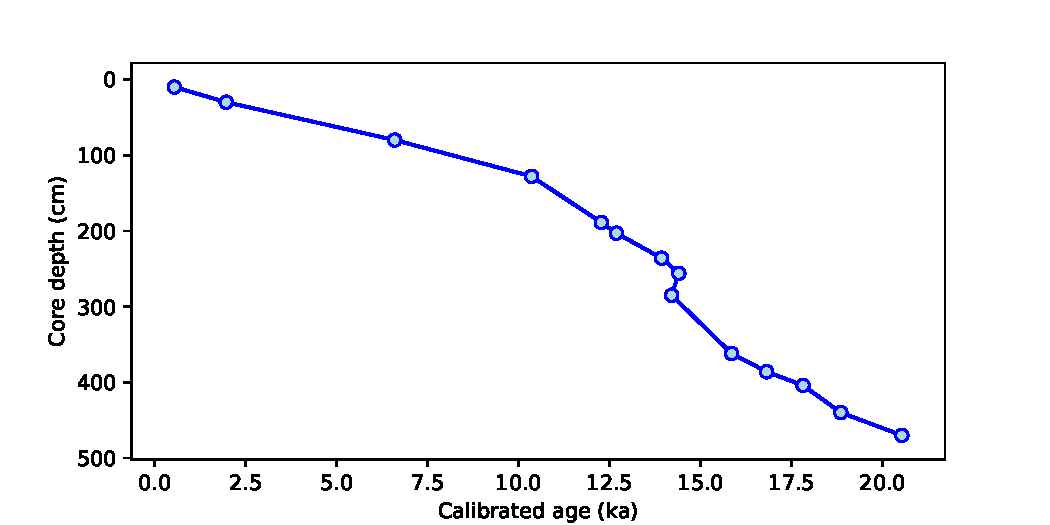
\includegraphics[width=\textwidth]{img/line_age_depth.pdf}
    \caption{Planktic foraminifera calibrated age against depth in sediment core OCE-326-GGC14, on the Laurentian fan.}
        \label{fig:age_depth}
\end{figure}

\subsection{Question 2}
\label{sec:Q2.2}

\begin{figure}[h]
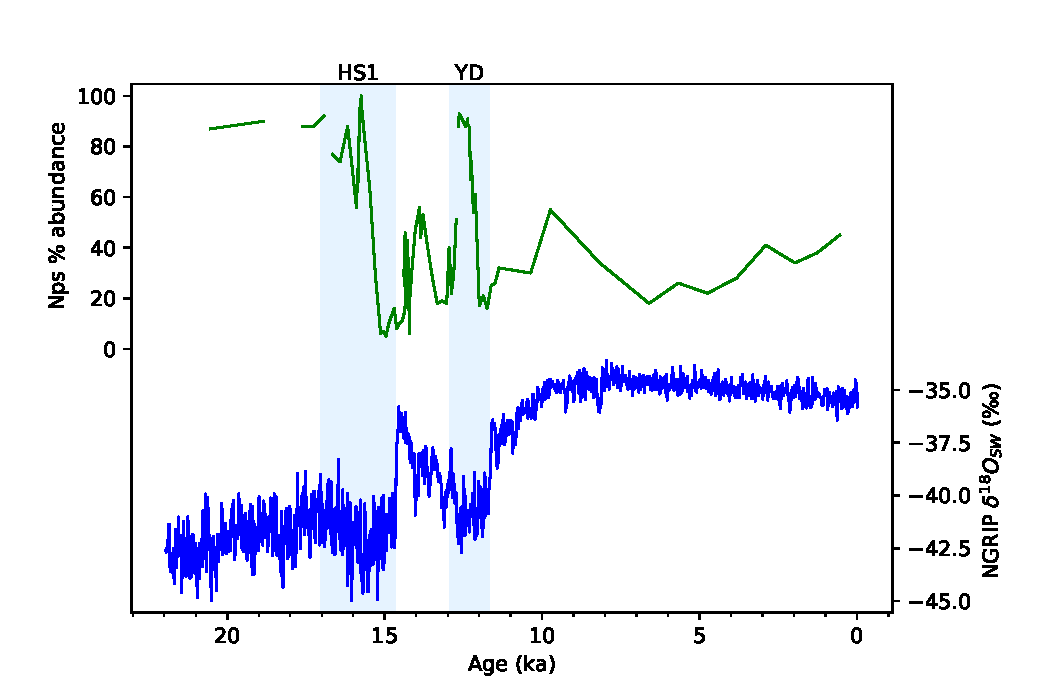
\includegraphics[width=\textwidth]{img/timeseries_nps_ngrip}
    \caption{Time series of abundance of planktic foraminifera \emph{N. pachyderma} sinistral (\emph{Nps}) in OCE-326-GGC14 (top) and oxygen isotope excursion in Greenland ice core NGRIP (bottom).}
        \label{fig:nps_ngrip}
\end{figure}

Figure \ref{fig:nps_ngrip} shows a strong antiphase relationship between \emph{Nps} abundance in the North Atlantic and \delO{} in Greenland, and both record abrupt climate cooling during the HS1 and YD stadials.
While changes in the latter appear to lag those in the former by approximately 0.5--1 ka, there is uncertainty in the calibration of foraminiferal $_{14}\mathrm{C}$ radiocarbon dates due to measurement error and, in particular, the assumption of a constant 400 year radiocarbon reservoir age --- a value that was likely higher during stadial events due to decreased ocean ventilation \parencite{bard1994north, hughen2004marine04}.
